
We return to the application of association screenings for categorical variables, and put the results in the previous section to use.
In particular, we focus on the exact-approximate support recovery problem, and demonstrate the consequences of its phase transition (Theorem \ref{thm:chi-squared-exact-approx-boundary}) in genetic association studies.

In order to do so, we must first connect the concept of   ``statistical signal size'' $\lambda$ with some key quantities in association tests.
While ``signal size'' likely sounds foreign to most practitioners, it is intimately linked with the concept of ``effect sizes'' --- or odds ratios --- in association studies, which are frequently estimated and reported in GWAS catalogs. This terminology, in turn, may be alien to some statisticians.  Here, we aim to clarify 
the two languages.

 %in Section \ref{sec:odds-and-power}.

% Unlike in additive models where the parameter $\mu$ has the interpretation of signal-to-noise ratios, the meaning of the signal sizes $\lambda$ in chi-square model is perhaps not as transparent.

\stilian{Recall the general setup of genetic association testing in Chapter \ref{sec:motivation-chisq}, where one wants to test 
for the effect (or lack thereof) of a specific gene on the occurrence of a disease.  A randomly drawn individual from the entire population 
is characterized by a pair $(P,G)$ of binary random variables, where $P$ encodes the phenotype and $G$, the genotype.  For example, in
the context of a specific study,  by phenotype we mean whether or not the individual has the disease (belongs to the Cases group) or is healthy 
(Controls group).  The genotype encodes whether or not the gene in question is expressed (Variant 1) or not (Variant 2). 
Table  \ref{tab:multinomial-counts} in the introduction summarizes the {\em counts} for all phenotype-genotype combinations
for the individuals in a given study sampled from the population. These counts can be assumed to follow a multinomial distribution, with probabilities 
given in the following Table \ref{tab:multinomial-probabilites}.  Notice that there are fundamental study design questions here since the counts will 
depend on the way individuals are recruited in the study.  For example, ``controlling'' the number of Cases or Controls (as opposed to sampling at
random from the population) will change the theoretical parameters (probabilities) of the multinomial model.  
These questions will be addressed in Section \ref{sec:optimal-design}  below.  

In this section, we characterize the relationship between the aforementioned ``signal size'' and ``odds-ratio'' parameterizations 
in the special, but fairly common case of association tests on 2-by-2 contingency tables.
}{\fbox{CHECK PLEASE}}
Consider a 2-by-2 multinomial distribution with marginal probabilities of phenotypes $(\phi_1, \phi_2)$ and genotypes $(\theta_1, \theta_2)$.
The \emph{probability} table (as opposed to the table of multinomial \emph{counts} in the introduction) is as follows.
\begin{table}[h]\label{tab:multinomial-probabilites}
\begin{center}
    \begin{tabular}{cccc}
    \hline
    & \multicolumn{2}{c}{Genotype} \\
    \cline{2-3}
    Probabilities & Variant 1 & Variant 2 & Total by phenotype \\
    \hline
    Cases & $\mu_{11}$ & $\mu_{12}$ & $\phi_1$ \\
    Controls & $\mu_{21}$ & $\mu_{22}$ & $\phi_2$ \\
    Total by genotype & $\theta_1$ & $\theta_2$ & 1 \\
    \hline
    \end{tabular}
    \caption{Probabilities of the multinomial distribution in a genetic association test. (Compare and contrast with 
    Table \ref{tab:multinomial-counts}. We have $\E[ O_{ij}] = n\mu_{ij},\ i,j=1,2$, where $n = \sum_{i,j} O_{ij}$.) }
\end{center}
\end{table}

The odds ratio (i.e., ``effect size'') is defined as the ratio of the phenotype frequencies between the two genotype variants,
\begin{equation} \label{eq:odds-ratio}
    \text{R} := \frac{\mu_{11}}{\mu_{21}}\Big/\frac{\mu_{12}}{\mu_{22}}
    = \frac{\mu_{11}\mu_{22}}{\mu_{12}\mu_{21}}.
\end{equation}
The multinomial distribution is fully parametrized by the trio $(\theta_1, \phi_1, R)$.
Odds ratios further away from 1 indicate greater contrasts between the probability of outcomes.
Independence between the genotypes and phenotypes would imply an odds ratio of one, and hence $\mu_{jk} = \phi_j\theta_k$, for all $j,k \in\{1,2\}$.

% When data are sampled from the multinomial distribution, the chi-square test defined in \eqref{eq:chisq-statistic} is asymptotically equivalent to tests including, e.g., the likelihood ratio test and Welch's t-test, both in terms of level and power \cite{ferguson2017course,gao2019upass}.
For a sequence of local alternatives $\mu^{(1)}, \mu^{(2)}, \ldots$, such that $\sqrt{n}(\mu^{(n)}_{jk} - \phi_j\theta_k)$ converges to a constant table $\delta = (\delta_{jk})$, the chi-square test statistics converge in distribution to the non-central chi-squared distribution with non-centrality parameter 
\begin{equation*}
    \lambda = \sum_{j=1}^2 \sum_{k=1}^2 {\delta_{jk}^2}/{(\phi_j\theta_k)}.
\end{equation*}
See, e.g., \cite{ferguson2017course}.
Hence, for large samples from a fixed distribution $(\mu_{ij})$, the statistic is well approximated by a $\chi^2_1(\lambda)$ distribution, where
\begin{equation} 
\lambda = n\sum_{j=1}^2 \sum_{k=1}^2 \frac{(\mu_{jk} - \phi_j\theta_k)^2}{\phi_j\theta_k}.
\end{equation}
%Since $\lambda$ is linear in the number of samples $n$, 
% Power of association tests at $\alpha$ level is approximately $\P[\chi^2_{\nu}(\lambda)>\chi^2_{\nu,\alpha}]$, where $\chi^2_{\nu,\alpha}$ is the upper $\alpha$-quantile of a central Chi-squared distribution.
Power calculations therefore only depend on the $\mu_{jk}$'s through $\lambda=nw^2$, where we define 
\begin{equation} \label{eq:signal-size-chisq}
    w^2:=\lambda/n
\end{equation} 
to be the \emph{signal size per sample}. 
Statistical power would be increasing in $w^2$ for fixed sample sizes.

The next proposition states that the statistical signal size per sample can be parametrized by the odds ratio and the marginals in the probability table.

\begin{proposition} \label{prop:signal-size-odds-ratio}
Consider a 2-by-2 multinomial distribution with marginal distributions $(\phi_1, \phi_2 = 1-\phi_2)$ and $(\theta_1, \theta_2=1-\theta_1)$.
Let signal size $w^2$ be defined as in \eqref{eq:signal-size-chisq}, and odds ratio $\text{R}$ be defined as in \eqref{eq:odds-ratio}. 
If $R=1$, we have $w^2 = 0$; if $R\in(0,1)\cup(1,+\infty)$, then we have
\begin{equation} \label{eq:signal-size-odds-ratio}
    w^2(\text{R}) =
    \frac{1}{4A(\text{R}-1)^2}\left(B+CR-\sqrt{(B+CR)^2-4A(R-1)^2}\right)^2,
\end{equation}
where $A = \phi_1\theta_1\phi_2\theta_2$, $B = \phi_1\theta_1+\phi_2\theta_2$, and $C = \phi_1\theta_2+\phi_2\theta_1$.
\end{proposition}

\begin{proof}
	We parametrize the 2-by-2 multinomial distribution with the parameter $\delta$, 
	\begin{equation} \label{eq:reparametrize-2-by-2-table-1}
	\mu_{11} = \phi_1\theta_1+\delta,\quad 
	\mu_{12} = \phi_1\theta_2-\delta,\quad 
	\mu_{21} = \phi_2\theta_1-\delta,\quad 
	\mu_{22} = \phi_2\theta_2+\delta.
	\end{equation}
	By relabelling of categories, we may assume $0<\theta_1,\phi_1\le1/2$ without loss of generality.
	Note that $\delta$ must lie within the range $[\delta_\mathrm{min}, \delta_\mathrm{max}]$, where
	$$
	\delta_\mathrm{min} := \max\{-\phi_1\theta_1, -\phi_2\theta_2, \phi_1\theta_2-1, \phi_2\theta_1-1\} 
	= -\phi_1\theta_1,
	$$
	and
	$$
	\delta_\mathrm{max} := \min\{1-\phi_1\theta_1, 1-\phi_2\theta_2, \phi_1\theta_2, \phi_2\theta_1\}
	= \min\{\phi_1\theta_2, \phi_2\theta_1\},
	$$
	in order for $\mu_{ij}\ge0$ for all $i,j\in \{1,2\}$.
	Under this parametrization, Relation \eqref{eq:odds-ratio} then becomes
	\begin{align} \label{eq:odds-ratio-delta}
	\text{R} = \frac{\mu_{11}\mu_{22}}{\mu_{12}\mu_{21}}
	= \frac{\phi_1\theta_1\phi_2\theta_2 + \delta(\phi_1\theta_1+\phi_2\theta_2)+\delta^2}{\phi_1\theta_1\phi_2\theta_2 - \delta(\phi_1\theta_2+\phi_2\theta_1)+\delta^2}
	= \frac{A +\delta B + \delta^2}{A -\delta C + \delta^2},
	\end{align}
	which is one-to-one and increasing in $\delta$ on $(\delta_\mathrm{min}, \delta_\mathrm{max})$.
	Equation \eqref{eq:signal-size-chisq} becomes
	\begin{equation} \label{eq:signal-size-chisq-delta}
	w^2 = \sum_{i=1}^2 \sum_{j=1}^2 \frac{(\mu_{ij} - \phi_i\theta_j)^2}{\phi_i\theta_j}
	= \delta^2\sum_i\sum_j \frac{1}{\phi_i\theta_j}
	= \frac{\delta^2}{\phi_1\theta_1\phi_2\theta_2},
	\end{equation}
	Solving for $\delta$ in \eqref{eq:odds-ratio-delta}, and plugging into the expression for signal size \eqref{eq:signal-size-chisq-delta} yields Relation \eqref{eq:signal-size-odds-ratio}.
	
	The other three cases ($1/2\le\theta_1,\phi_1\le1$; $0<\theta_1\le1/2\le\phi_1\le1$; and $0\le\phi_1\le1/2\le\theta_1\le1$) may be obtained similarly, or by appealing to the symmetry of the problem.
\end{proof}

To understand Proposition \ref{prop:signal-size-odds-ratio}, we illustrate Relation \eqref{eq:signal-size-odds-ratio} for selected values of marginals $\theta_1$ and $\phi_1$ in Figure \ref{fig:signal-vs-odds}.
Observe in the figure that an odds ratio further away from one corresponds to stronger statistical signal per sample, ceteris paribus.
However, this ``valley'' pattern is in general not symmetric around 1, except for balanced marginal distributions ($\phi_1=1/2$ or $\theta_1=1/2$).
While the odds ratio $R$ can be arbitrarily close to 0 or diverge to $+\infty$ for any marginal distribution, the signal sizes $w^2$ are bounded from above by constants that depend only on the marginals.
% This is quantified in the next corollary.

\begin{figure}
      \centering
      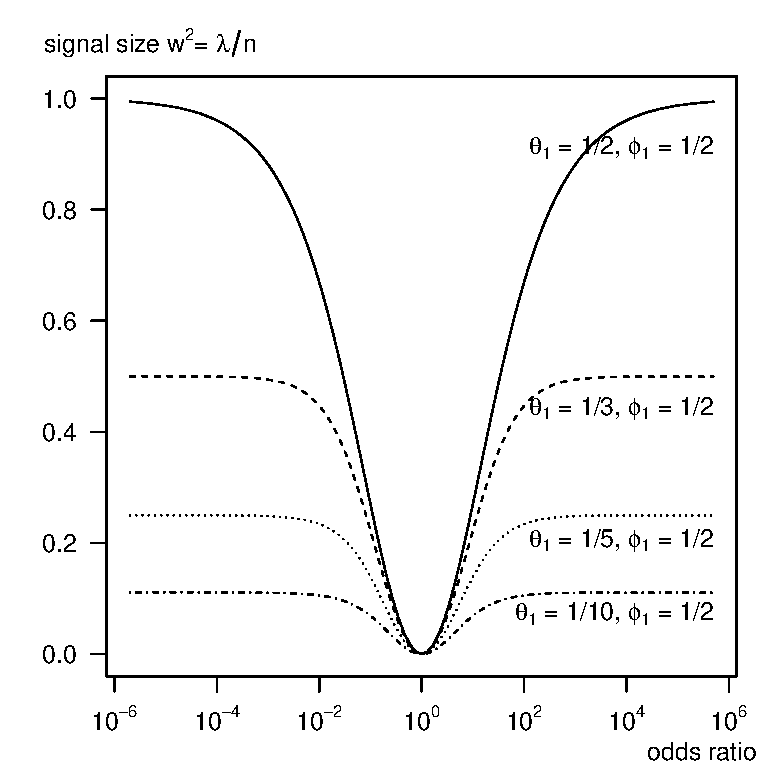
\includegraphics[width=0.49\textwidth]{pics/singal-vs-odds-p05}
      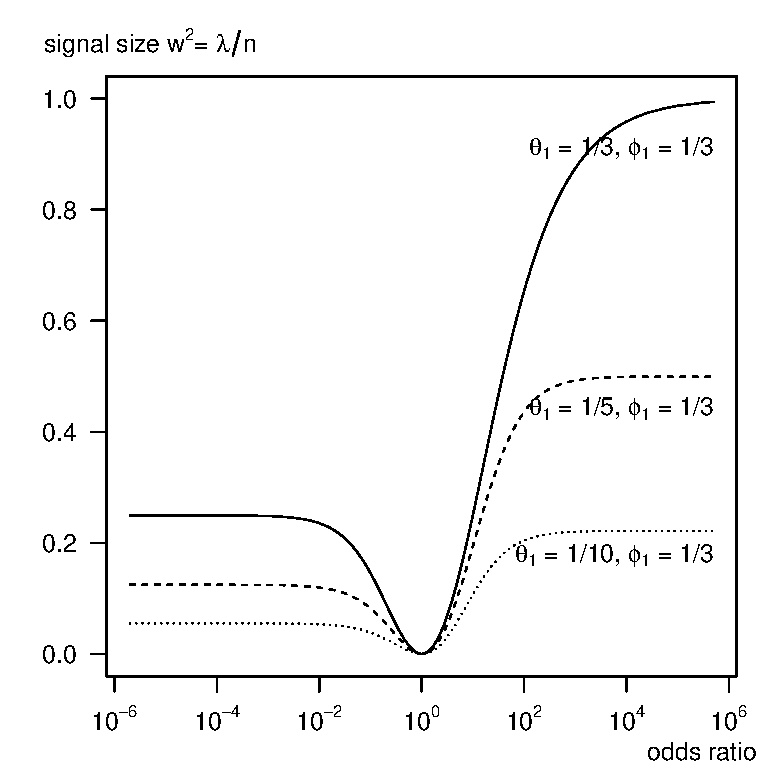
\includegraphics[width=0.49\textwidth]{pics/singal-vs-odds-p0333}            
      \caption{Signal sizes per sample $w^2$ as functions of odds ratios in 2-by-2 multinomial distributions for selected genotype marginals in balanced (left) and unbalanced (right) designs; see Relation \eqref{eq:signal-size-odds-ratio} in Proposition \ref{prop:signal-size-odds-ratio}. For given marginal distributions, extreme odds ratios imply stronger statistical signals at a given sample size. However, the signal sizes are bounded above by constants that depend on the marginal distributions; see Relations \eqref{eq:signal-size-upper-bound-1} and \eqref{eq:signal-size-upper-bound-2}. % Unbalanced marginal distributions -- or rare variants -- lead to smaller signal sizes at a given odds ratio.
      } 
      \label{fig:signal-vs-odds}
\end{figure}

\begin{corollary} \label{cor:signal-limits-OR}
The signal size as a function of the odds ratio $w^2(R)$ is decreasing on $(0,1)$ and increasing on $(1,\infty)$, with limits
\begin{equation} \label{eq:signal-size-upper-bound-1}
    \lim_{\text{R}\to0_+} w^2(\text{R}) = \min\left\{\frac{\phi_1\theta_1}{\phi_2\theta_2}, \frac{\phi_2\theta_2}{\phi_1\theta_1}\right\},
\end{equation}
and
\begin{equation} \label{eq:signal-size-upper-bound-2}
    \lim_{\text{R}\to+\infty} w^2(\text{R}) = \min\left\{\frac{\phi_1\theta_2}{\phi_2\theta_1}, \frac{\phi_2\theta_1}{\phi_1\theta_2}\right\}.
\end{equation}
\end{corollary}
% Proof of Corollary \ref{cor:signal-limits-OR} is found in Appendix \ref{sec:proof-signal-size-odds-ratio}. 

\begin{proof}
	As in the proof of Proposition \ref{prop:signal-size-odds-ratio}, we examine the case where $0<\theta_1,\phi_1\le1/2$, and leave the other three cases an exercise.
	Take the first derivative of the expression for $w^2$ in equation \eqref{eq:signal-size-chisq-delta} with respect to $\delta$, it is evident that $w^2(\delta)$ is decreasing on $[\delta_\mathrm{min},0)$, increasing on $(0,\delta_\mathrm{max}]$, with limits
	$$
	\lim_{d\to \delta_\mathrm{min}} w^2(\delta) = \frac{\phi_1\theta_1}{\phi_2\theta_2},
	\quad
	\text{and}
	\quad
	\lim_{d\to \delta_\mathrm{max}} w^2(\delta) = \min\left\{\frac{\phi_1\theta_2}{\phi_2\theta_1}, \frac{\phi_2\theta_1}{\phi_1\theta_2}\right\}.
	$$
\end{proof}

Corollary \ref{cor:signal-limits-OR} immediately implies that balanced designs with roughly equal number of cases and controls are not necessarily the most informative.

For example, in a study where a third of the recruited subjects carry the genetic variant positively correlated with the trait (i.e., $\theta_1=1/3$), an unbalanced design with $\phi_1=1/3$ would maximize $w^2$ at large odds ratios.
This unbalanced design is much more efficient compared to, say, a balanced design with $\phi_1=1/2$.
In the first case, we have $w^2\to1$ as $R\to\infty$; whereas in the second design, $w^2<1/2$ no matter how large $R$ is.
This difference can also be read by comparing the dashed curve ($\theta_1=1/3$, $\phi_1=1/2$) in the left panel of Figure \ref{fig:signal-vs-odds}, with the solid curve ($\theta_1=1/3$, $\phi_1=1/3$) in the right panel of Figure \ref{fig:signal-vs-odds}.
